%%=====================================================================================%%
%% Springer Nature Journal Article Manuscript (sn-jnl v3, sn-mathphys-num)             %%
%% Target Journal: General Relativity and Gravitation (Springer)                       %%
%%=====================================================================================%%
\documentclass[pdflatex,sn-mathphys-num]{sn-jnl}

\usepackage{graphicx}
\usepackage{multirow}
\usepackage{amsmath,amssymb,amsfonts}
\usepackage{amsthm}
\usepackage{mathrsfs}
\usepackage[title]{appendix}
\usepackage{xcolor}
\usepackage{textcomp}
\usepackage{manyfoot}
\usepackage{booktabs}

\theoremstyle{thmstyleone}
\newtheorem{theorem}{Theorem}
\newtheorem{proposition}[theorem]{Proposition}
\newtheorem{lemma}[theorem]{Lemma}

\theoremstyle{thmstyletwo}
\newtheorem{remark}{Remark}

\theoremstyle{thmstylethree}
\newtheorem{definition}{Definition}

\raggedbottom

\begin{document}

\title[Orientation-Reversing Regular Bounce and Variational Cosmological Budgets]{Orientation-Reversing Regular Bounce Geometry, Open-Horizon Variational Budgets, and Three-Axis Harmonic Freeze-Out in Nested Spacetimes}

\author*[1]{\fnm{Douglas} \sur{Ek}}\email{douglas@swedishsoftwareengineers.com}

\affil*[1]{\orgname{Independent Researcher}, \orgaddress{\city{B{\aa}stad}, \country{Sweden}} (ORCID: \href{https://orcid.org/0009-0003-2422-6098}{0009-0003-2422-6098})}

\abstract{Standard gravitational collapse and Friedmann--Lema\^{i}tre--Robertson--Walker (FLRW) models typically impose two independent structural assumptions: restriction of the areal coordinate to an unsigned radial half-line $r \ge 0$, and adiabatic isolation of the expanding cosmological interior as a closed thermodynamic system. Motivated by isotropic-singularity frameworks, conformal cyclic cosmology, and regular black-bounce geometries, we analyze a two-sheeted spacetime continuation in which a signed radial coordinate $R \in (-\infty,\infty)$ crosses smoothly through a regular throat $\Sigma_0$ ($R=0$) of minimum core radius $R_{\mathrm{core}} = \sqrt{2\pi/\kappa} > 0$ and hybrid radial metric factor $M(R) = (1 + R^2/3)^{-1}$. We prove that the resulting four-dimensional curvature invariants and orthonormal Einstein tensor components remain real-analytic and uniformly bounded across $\Sigma_0$, while orientation reverses on a single throat passage ($\det F = (R/R_0)^3$) and is restored across two successive passages. Reducing a covariant scalar-gravity action onto quantized one-dimensional vortex-phase bundles immersed in a parent vacuum energy density $P \equiv V(s_\star)$ yields a five-variable variational energy functional across $\Sigma_0$. Eliminating the internal stationarity variables produces an exact, parameter-free cubic relation $9DVB = 4(V + B/2)^3$ among the dimensionless vacuum-stretch ($D = \Omega_{\mathrm{DE}}$), boundary-dust ($M = \Omega_{\mathrm{DM}}$), and visible-filament ($V = \Omega_{\mathrm{vis}}$) density shares, with $B = M - D/3$. Natural boundary variation across an unpinned throat enforces winding chemical-potential equilibrium $\mu_+ = \mu_-$ and yields an effective open-system vacuum equation of state $w_{\mathrm{DE}} = -1$ ($\rho_{\mathrm{DE}} = 3P = \mathrm{const}$) alongside pressureless boundary dust ($w_{\mathrm{DM}} = 0$), while leaving the overall dimensional scale $P$ (and thus the absolute value of $\Lambda = 3\kappa P$) as the single free scale of the effective action. Finally, solving the whole-exterior harmonic two-center neck instability yields the exact characteristic cubic $p^3 - 3p - 3 = 0$ with unstable growth root $p_+ = \varphi^{2/3} + \varphi^{-2/3} \approx 2.103803$, whose Laplace trace-zero cascade ($\Delta\Phi = 0$) exhausts the three orthogonal spatial axes at logarithmic compression depth $\chi_{\mathrm{freeze}} = 3$. Evaluating the invariant budget curve at $\Omega_b = e^{-3} = 0.04979$ selects $(\Omega_{\mathrm{DE}}, \Omega_{\mathrm{DM}}, \Omega_b) = (0.7114, 0.2388, 0.0498)$ without adjustable partition parameters; calibrating the physical scale solely against the cosmic microwave background baryon density $\omega_b = 0.02237 \pm 0.00015$ yields $H_0 = 67.03 \pm 0.22\ \mathrm{km\,s^{-1}\,Mpc^{-1}}$ and suppresses late-time sub-horizon clustering via a $3.11\%$ uncondensed filament fraction to $S_8 \approx 0.776$.}

\keywords{Regular black-hole bounce, Isotropic singularities, Open-horizon thermodynamics, Cosmological density parameters, Harmonic multipole instability, Hubble and $S_8$ tensions}

\pacs[MSC Classification]{83C75, 83F05, 58J32, 35J05}

\maketitle

\section{Introduction}\label{sec:intro}

The classical singularity theorems of Penrose and Hawking establish that, under generic trapping and energy conditions on a single Lorentzian manifold, causal geodesics become incomplete in gravitational collapse and in the cosmological past \cite{Penrose1965,HawkingPenrose1970}. Whether geodesic incompleteness signals an absolute boundary of physical spacetime or a breakdown of unsigned coordinate charts and effective matter approximations has been investigated along three distinct mathematical avenues. First, in the isotropic-singularity programme developed by Goode, Wainwright, Anguige, and Tod \cite{GoodeWainwright1985,AnguigeTod1999,Tod2003} and extended in Penrose's Conformal Cyclic Cosmology (CCC) \cite{Penrose2010,Tod2015,GurzadyanPenrose2013}, cosmological initial data are regularized by conformal rescaling across a smooth three-surface separating successive cosmic domains. Second, regular black-hole and ``black-universe'' constructions---originating from the two-sheeted bridge of Einstein and Rosen \cite{EinsteinRosen1935} and developed by Frolov, Markov, and Mukhanov \cite{FrolovMarkovMukhanov1990}, Smolin \cite{Smolin1992}, Bronnikov and collaborators \cite{Bronnikov2007,BronnikovDonskoy2010}, Pop{\l}awski \cite{Poplawski2010,Poplawski2012}, and Simpson and Visser \cite{MorrisThorne1988,SimpsonVisser2019,CarballoRubio2020}---replace the singular $r=0$ center by a minimum throat scale $R_{\mathrm{core}} > 0$ opening into an expanding interior region, closely related to smooth degenerate-metric extensions \cite{KossowskiKriele1993}. Third, open-system horizon thermodynamics---following Israel's hypersurface formalism \cite{Israel1966}, Gibbons and Hawking \cite{GibbonsHawking1977}, Jacobson \cite{Jacobson1995}, Prigogine et al.\ \cite{Prigogine1989}, and Lima \cite{Lima1996}---demonstrates that continuous entropy or mode transfer across a bounding horizon produces an effective negative creation pressure in the interior Friedmann continuity equation without introducing exotic closed-box phantom or quintessence fluids.

Despite extensive progress within each of these three programmes individually, an important quantitative gap has remained open: \emph{when a parent gravitational collapse couples across a regular throat $\Sigma_0$ into an expanding interior domain, does a single variational principle relate the regular bounce geometry at $\Sigma_0$, the effective equations of state $(w_{\mathrm{DE}}, w_{\mathrm{DM}}, w_b)$, and the observed dimensionless cosmological partition $(\Omega_{\mathrm{DE}}, \Omega_{\mathrm{DM}}, \Omega_b)$?} In standard flat $\Lambda$CDM cosmology, $\Omega_\Lambda$, $\Omega_c$, and $\Omega_b$ are independent free parameters fitted a posteriori to cosmic microwave background (CMB) and baryon acoustic oscillation (BAO) observations \cite{Planck2018,ACTDR6_2024,DESI2024}, while the absolute magnitude of the cosmological constant $\Lambda$ remains unexplained \cite{Weinberg1989} and mild but persistent tensions appear between early-universe CMB extrapolations and late-universe weak-lensing measurements of the clustering amplitude $S_8 \equiv \sigma_8\sqrt{\Omega_m/0.3}$ \cite{KiDS1000_2021,DESY3_KiDS_2023}.

In this paper, we formulate and analyze a compact variational and differential-geometric framework---\emph{Nested-Space Cosmology} (NSC)---that connects these three threads within an explicitly scoped mathematical model. To maintain strict epistemic clarity regarding what is derived and what remains open, we state our scope upfront:
\begin{enumerate}
\item \textbf{Free dimensional scale ($\Lambda$ remains open):} The parent background scalar potential minimum $P \equiv V(s_\star) > 0$ sets the overall dimensional energy-density scale of the interior vacuum component ($\rho_{\mathrm{DE}} = 3P$, i.e., $\Lambda_{\mathrm{eff}} = 3\kappa P$ with $\kappa = 8\pi G/c^4$). We do \emph{not} claim a first-principles derivation of the numerical magnitude of $\Lambda$ in Planck units; resolving the $10^{-122}$ hierarchy between $P$ and the Planck energy density remains an open boundary-value problem \cite{Weinberg1989}.
\item \textbf{Parameter-free dimensionless ratios:} Once $P$ and the reference topological winding stiffness $m_0$ are factored out by normalization, minimizing the reduced five-variable variational cost functional across the throat $\Sigma_0$ eliminates \emph{both} internal state variables $(\theta^\star, \chi)$ and confines the dimensionless density fractions $(D, M, V) = (\Omega_{\mathrm{DE}}, \Omega_{\mathrm{DM}}, \Omega_{\mathrm{vis}})$ to an exact parameter-free algebraic curve, $9DVB = 4(V + B/2)^3$ with $B = M - D/3$.
\item \textbf{Single empirical calibration for $H_0$:} Combining a three-axis harmonic neck-splitting cascade ($\Delta\Phi = 0$) with integer logarithmic winding quantization fixes the cascade termination depth at $\chi_{\mathrm{freeze}} = 3$ and the condensed baryon share at $\Omega_b = e^{-3} \approx 0.049787$. Supplying the single empirical BBN/CMB physical baryon density $\omega_b \equiv \Omega_b h^2 = 0.02237 \pm 0.00015$ \cite{Planck2018} then determines $H_0 = 100\sqrt{\omega_b e^3} = 67.03 \pm 0.22\ \mathrm{km\,s^{-1}\,Mpc^{-1}}$ and predicts late-time $S_8$ suppression without adjustable cosmological fit parameters.
\end{enumerate}

The paper is organized as follows. Section~\ref{sec:bounce} introduces the phase-accumulation metric generator, compares signed and unsigned radial continuations across a degenerate throat $\Sigma_0$, and proves analyticity and curvature boundedness of the two-sheeted regular bounce metric (Propositions~\ref{prop:bounce} and \ref{prop:bianchi}). Section~\ref{sec:variational} derives the reduced five-variable variational functional from a covariant 3+1D scalar-gravity action (Propositions~\ref{prop:reduction} and \ref{prop:junction}) and proves Theorem~\ref{thm:budget} establishing the exact cubic budget surface $9DVB = 4(V + B/2)^3$ and the open-horizon equations of state $w_{\mathrm{DE}} = -1$ and $w_{\mathrm{DM}} = 0$. Section~\ref{sec:triad} establishes the three-dimensional $(1,1,1)$ standing-wave ground state, its hard-core merger barrier, and the Gauss-divergence $3:1$ exterior potential-flow partition (Theorems~\ref{thm:triad} and \ref{thm:virial}). Section~\ref{sec:cascade} derives the whole-exterior two-center neck instability cubic $p^3 - 3p - 3 = 0$, the Laplace trace-zero three-axis orthogonal cascade, topological freeze-out at $\chi_{\mathrm{freeze}} = 3$, and the observational readouts for $\Omega_{\mathrm{DE}}$, $\Omega_{\mathrm{DM}}$, $\Omega_b$, the warm--hot intergalactic medium (WHIM) fraction, $H_0$, and $S_8$ (Theorems~\ref{thm:neck}--\ref{thm:freeze} and Proposition~\ref{prop:observables}). Section~\ref{sec:discussion} summarizes falsifiable observational tests and open theoretical problems.

\section{Orientation-Reversing Continuation and Regular Bounce Geometry}\label{sec:bounce}

\subsection{Discrete Phase-Offset Generator and Metric Completion}\label{subsec:generator}

Before introducing four-dimensional Lorentzian curvature, we note the elementary kinematic motivation for two-sheeted radial coordinates. Consider a discrete two-stage phase accumulator driven by a single real increment $\alpha \in \mathbb{R}\setminus\mathbb{Q}$:
\begin{equation}\label{eq:weyl_map}
\theta_{n+1} = \theta_n + \alpha \pmod{1}, \qquad \phi_{n+1} = \phi_n + \theta_n \pmod{1}, \qquad \theta_0 = \phi_0 = 0,
\end{equation}
so that $\theta_n = n\alpha$ and $\phi_n = \frac{1}{2}n(n-1)\alpha \pmod{1}$. By Weyl's polynomial equidistribution theorem \cite{Weyl1916}, the sequence $(\Theta_n, \Phi_n) = (2\pi\theta_n, 2\pi\phi_n)$ is dense on $\mathbb{T}^2$, generating unit directions $v_n = (\sin\Theta_n\cos\Phi_n, \sin\Theta_n\sin\Phi_n, \cos\Theta_n) \in S^2$ with inner-product kernel $C_{nm} = v_n \cdot v_m$. Endowing a radial interval with the Euclidean law of cosines $d^2[(r,n),(s,m)] = r^2 + s^2 - 2rs C_{nm}$ (or the spherical law $\cos(d/R) = \cos(r/R)\cos(s/R) + \sin(r/R)\sin(s/R)C_{nm}$) yields the closed ball $B^3$ (or $S^3$) as metric completion \cite{Ek2026Zenodo}.

Projected onto any diameter of a closed circular phase orbit $z(\tau) = R_0 e^{i\omega\tau}$, uniform phase progression satisfies the harmonic oscillator equation
\begin{equation}\label{eq:signed_pendulum}
R(\tau) = \mathrm{Re}\!\left(R_0 e^{i\omega\tau}\right) = R_0 \cos(\omega\tau), \qquad \ddot{R} + \omega^2 R = 0,
\end{equation}
with conserved invariant $\frac{1}{2}\dot{R}^2 + \frac{1}{2}\omega^2 R^2 = \frac{1}{2}R_0^2\omega^2$. If the radial coordinate is restricted a priori to an unsigned half-line $r(\tau) \equiv |R(\tau)| \ge 0$, folding the negative half-cycle ($R < 0$) onto $r \ge 0$ introduces an artificial velocity discontinuity and distributional acceleration singular support at the crossing time $\tau_0 = \pi/(2\omega)$ ($R=0$):
\begin{equation}\label{eq:unsigned_cusp}
\Delta\dot{r} \equiv \dot{r}(\tau_0^+) - \dot{r}(\tau_0^-) = +2R_0\omega, \qquad \ddot{r}(\tau) = 2R_0\omega\,\delta(\tau - \tau_0) - \omega^2 r(\tau).
\end{equation}
Retaining the signed coordinate $R \in (-\infty,\infty)$ eliminates this kinematic cusp identically ($\Delta\dot{R} = 0$, $\ddot{R}(\tau_0) = 0$). In $d=3$ spatial dimensions, the isotropic spatial Jacobian across $\Sigma_0 = \{R=0\}$,
\begin{equation}\label{eq:jacobian_flip}
\det F = \det\!\left[\left(\frac{R}{R_0}\right) I_3\right] = \left(\frac{R}{R_0}\right)^3,
\end{equation}
changes sign smoothly from $\mathcal{M}_+$ ($R > 0$, $\det F > 0$) to $\mathcal{M}_-$ ($R < 0$, $\det F < 0$), converting parent contraction ($\dot{R} < 0$) into outward interior expansion ($\dot{r}_- = -\dot{R} > 0$ for $r_- \equiv -R > 0$), as studied in degenerate-metric extensions of general relativity \cite{KossowskiKriele1993}. Crucially, because spatial parity inversion $\mathcal{P} = -I_3$ satisfies $\det\mathcal{P} = (-1)^3 = -1$, two successive throat passages restore orientation identically: $\mathcal{P}^2 = (-I_3)^2 = +I_3$ with $\det(\mathcal{P}^2) = +1$ (Fig.~\ref{fig:bounce}a).

\begin{figure}[t]
\centering
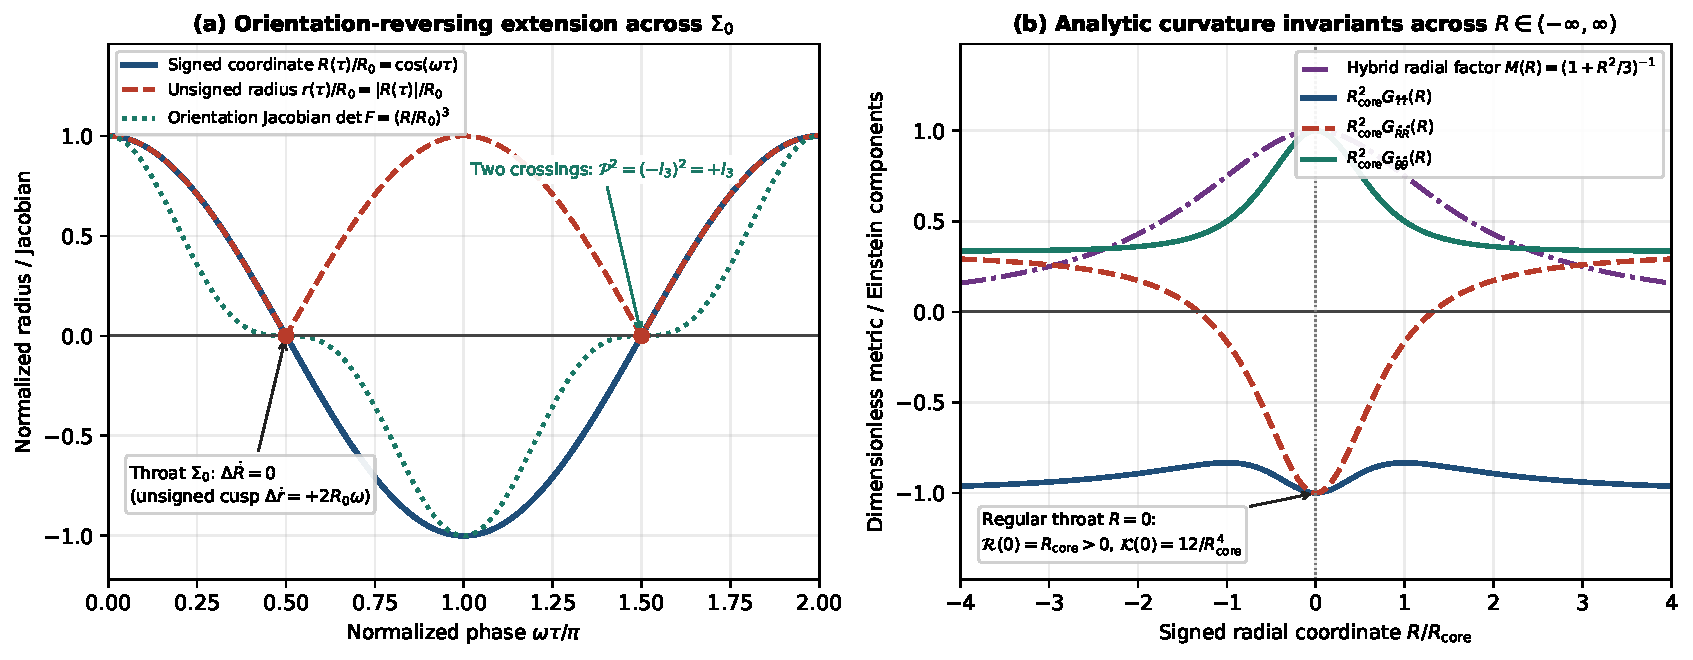
\includegraphics[width=\textwidth]{figures/fig1-bounce-and-geometry.pdf}
\caption{\textbf{Orientation-reversing radial extension and regular bounce curvature.} \textbf{(a)} Comparison of the smooth signed trajectory $R(\tau)/R_0 = \cos(\omega\tau)$ and three-dimensional orientation Jacobian $\det F = (R/R_0)^3$ against the artificial velocity cusp $\Delta\dot{r} = +2R_0\omega$ induced by restricting radius to $r = |R| \ge 0$; two successive throat crossings restore spatial orientation ($\mathcal{P}^2 = +I_3$). \textbf{(b)} Analytic behavior of the hybrid radial metric coefficient $M(R) = (1+R^2/3)^{-1}$ and dimensionless orthonormal Einstein tensor components $R_{\mathrm{core}}^2 G_{\hat{a}\hat{b}}(R)$ across the regular throat $R=0$ (Proposition~\ref{prop:bianchi}).}\label{fig:bounce}
\end{figure}

\subsection{Analytic Two-Sheeted Bounce Metric and Curvature Regularity}\label{subsec:regular_metric}

In curved 3+1D spacetime, simply setting the areal radius equal to $|R|$ still leaves $S^2$ spheres shrinking to zero area at $R=0$. However, when standing-wave phase modes carry a minimum core scale $R_{\mathrm{core}} > 0$ (derived from the $(1,1,1)$ cavity ground state in Section~\ref{sec:triad}) and hybrid radial inertia $M(R) = (1 + R^2/3)^{-1}$ (which simultaneously ensures finite proper birth distance $\int_0^\varepsilon \sqrt{M(R)}\,dR < \infty$ near $R=0$ and finite conformal optical reach $\int^\infty \sqrt{M(R)}\,dR/R < \infty$ at large $|R|$), we obtain a regular two-sheeted generalization of the Simpson--Visser black-bounce geometry \cite{SimpsonVisser2019,Bronnikov2007}.

\begin{proposition}[Regular Two-Sheeted Bounce Line Element]\label{prop:bounce}
Let $\mathcal{M} = \mathbb{R}_\tau \times \mathbb{R}_R \times S^2$ carry the Lorentzian line element (in units $c=1$, $\kappa = 8\pi G$)
\begin{equation}\label{eq:bounce_metric}
ds^2 = -d\tau^2 + M(R)\,dR^2 + \mathcal{R}^2(R)\,d\Omega_2^2, \quad \mathcal{R}(R) \equiv \sqrt{R^2 + R_{\mathrm{core}}^2}, \quad M(R) \equiv \frac{1}{1 + R^2/3},
\end{equation}
with $R_{\mathrm{core}} = \sqrt{2\pi/\kappa} > 0$. Then $g_{\mu\nu}$ is $C^\infty$ and non-degenerate for all $R \in (-\infty,\infty)$, with minimum throat area $A_{\min} = 4\pi R_{\mathrm{core}}^2$ at $\Sigma_0 = \{R=0\}$, and bounded Ricci and Kretschmann scalars at $R=0$:
\begin{equation}\label{eq:bounce_invariants}
R_4(0) = -\frac{2}{R_{\mathrm{core}}^2} = -\frac{\kappa}{\pi} < \infty, \qquad \mathcal{K}_{\mathrm{static}}(0) = R_{\mu\nu\rho\sigma}R^{\mu\nu\rho\sigma}\Big|_{R=0} = \frac{12}{R_{\mathrm{core}}^4} = \frac{3\kappa^2}{\pi^2} < \infty.
\end{equation}
If the throat oscillates harmonically at $R(\tau) = R_0\cos(\omega\tau)$, the dynamical Kretschmann scalar at crossing satisfies $\mathcal{K}_{\mathrm{dyn}}(0) = \frac{3\kappa^2}{\pi^2}(1 + R_0^2\omega^2)^2 < \infty$.
\end{proposition}

\begin{proof}
At $R=0$, $M(0) = 1$, $M'(0) = 0$, $M''(0) = -2/3$, $\mathcal{R}(0) = R_{\mathrm{core}} > 0$, $\mathcal{R}'(0) = 0$, and $\mathcal{R}''(0) = 1/R_{\mathrm{core}}$. Introducing the orthonormal coframe $\omega^{\hat{\tau}} = d\tau$, $\omega^{\hat{R}} = \sqrt{M(R)}\,dR$, $\omega^{\hat{\theta}} = \mathcal{R}(R)\,d\theta$, and $\omega^{\hat{\phi}} = \mathcal{R}(R)\sin\theta\,d\phi$, Cartan's structure equations give the non-vanishing orthonormal Riemann components for all $R \in (-\infty,\infty)$:
\begin{align}
R_{\hat{R}\hat{\theta}\hat{R}\hat{\theta}}(R) &= R_{\hat{R}\hat{\phi}\hat{R}\hat{\phi}}(R) = -\frac{\mathcal{R}''}{M\mathcal{R}} + \frac{M'\mathcal{R}'}{2M^2\mathcal{R}} = -\frac{R_{\mathrm{core}}^2(1 + R^2/3) + \frac{1}{3}R^2(R^2 + R_{\mathrm{core}}^2)}{(R^2 + R_{\mathrm{core}}^2)^2}, \label{eq:riem_rtheta}\\
R_{\hat{\theta}\hat{\phi}\hat{\theta}\hat{\phi}}(R) &= \frac{1}{\mathcal{R}^2} - \frac{(\mathcal{R}')^2}{M\mathcal{R}^2} = \frac{R_{\mathrm{core}}^2 - R^4/3}{(R^2 + R_{\mathrm{core}}^2)^2}. \label{eq:riem_thetaphi}
\end{align}
Evaluating Eqs.~\eqref{eq:riem_rtheta}--\eqref{eq:riem_thetaphi} at $R=0$ gives $R_{\hat{R}\hat{\theta}\hat{R}\hat{\theta}}(0) = R_{\hat{R}\hat{\phi}\hat{R}\hat{\phi}}(0) = -1/R_{\mathrm{core}}^2$ and $R_{\hat{\theta}\hat{\phi}\hat{\theta}\hat{\phi}}(0) = +1/R_{\mathrm{core}}^2$. Contracting yields $R_4(0) = 2(-2/R_{\mathrm{core}}^2 + 1/R_{\mathrm{core}}^2) = -2/R_{\mathrm{core}}^2$ and $\mathcal{K}_{\mathrm{static}}(0) = 4\big[2(-1/R_{\mathrm{core}}^2)^2 + (+1/R_{\mathrm{core}}^2)^2\big] = 12/R_{\mathrm{core}}^4$. Including $\dot{R}(\tau_0) = \mp R_0\omega$ scales each spatial curvature principal value by $(1 + R_0^2\omega^2)$, giving $\mathcal{K}_{\mathrm{dyn}}(0) = \frac{3\kappa^2}{\pi^2}(1 + R_0^2\omega^2)^2$.
\end{proof}

\begin{proposition}[Orthonormal Einstein Tensor and Contracted Bianchi Identity Across $\Sigma_0$]\label{prop:bianchi}
For the metric~\eqref{eq:bounce_metric}, the orthonormal Einstein tensor $G_{\hat{a}\hat{b}}(R) = \kappa T_{\hat{a}\hat{b}}(R)$ is analytic everywhere on $R \in (-\infty,\infty)$ and is given explicitly by
\begin{align}
G_{\hat{\tau}\hat{\tau}}(R) &= -\frac{R^4 + \frac{4}{3}R^2 R_{\mathrm{core}}^2 + R_{\mathrm{core}}^2}{(R^2 + R_{\mathrm{core}}^2)^2}, \qquad
G_{\hat{R}\hat{R}}(R) = \frac{\frac{1}{3}R^4 - R_{\mathrm{core}}^2}{(R^2 + R_{\mathrm{core}}^2)^2}, \label{eq:einstein_tt_rr}\\
G_{\hat{\theta}\hat{\theta}}(R) &= G_{\hat{\phi}\hat{\phi}}(R) = \frac{\frac{1}{3}R^4 + \frac{2}{3}R^2 R_{\mathrm{core}}^2 + R_{\mathrm{core}}^2}{(R^2 + R_{\mathrm{core}}^2)^2}. \label{eq:einstein_thth}
\end{align}
At the throat $R=0$, $G_{\hat{a}\hat{b}}(0) = R_{\mathrm{core}}^{-2}\,\mathrm{diag}(-1, -1, +1, +1)$, so $\rho_{\mathrm{eff}}(0) + p_{R,\mathrm{eff}}(0) = \kappa^{-1}[G_{\hat{\tau}\hat{\tau}}(0) + G_{\hat{R}\hat{R}}(0)] = -2/(\kappa R_{\mathrm{core}}^2) < 0$, satisfying the standard flare-out condition of regular black-bounce throats \cite{MorrisThorne1988,SimpsonVisser2019} via radial Casimir-like winding tension while satisfying the radial Bianchi conservation identity $\frac{d}{dR}G_{\hat{R}\hat{R}} + \frac{2\mathcal{R}'}{\mathcal{R}}(G_{\hat{R}\hat{R}} - G_{\hat{\theta}\hat{\theta}}) = 0$ identically (Fig.~\ref{fig:bounce}b).
\end{proposition}

\begin{proof}
In an orthonormal static spherically symmetric frame with signature $(-,+,+,+)$, $G_{\hat{\tau}\hat{\tau}} = -(2R_{\hat{R}\hat{\theta}\hat{R}\hat{\theta}} + R_{\hat{\theta}\hat{\phi}\hat{\theta}\hat{\phi}})$, $G_{\hat{R}\hat{R}} = -R_{\hat{\theta}\hat{\phi}\hat{\theta}\hat{\phi}}$, and $G_{\hat{\theta}\hat{\theta}} = G_{\hat{\phi}\hat{\phi}} = -R_{\hat{R}\hat{\theta}\hat{R}\hat{\theta}}$. Substituting Eqs.~\eqref{eq:riem_rtheta}--\eqref{eq:riem_thetaphi} gives $2R_{\hat{R}\hat{\theta}\hat{R}\hat{\theta}} + R_{\hat{\theta}\hat{\phi}\hat{\theta}\hat{\phi}} = [-2R_{\mathrm{core}}^2 - \frac{4}{3}R^2 R_{\mathrm{core}}^2 - \frac{2}{3}R^4 + R_{\mathrm{core}}^2 - \frac{1}{3}R^4]/\mathcal{R}^4 = -[R^4 + \frac{4}{3}R^2 R_{\mathrm{core}}^2 + R_{\mathrm{core}}^2]/\mathcal{R}^4$, yielding Eqs.~\eqref{eq:einstein_tt_rr}--\eqref{eq:einstein_thth}. Direct differentiation gives $\frac{d}{dR}G_{\hat{R}\hat{R}} = \frac{4R(R^2 + 3)R_{\mathrm{core}}^2}{3(R^2 + R_{\mathrm{core}}^2)^3}$ and $\frac{2\mathcal{R}'}{\mathcal{R}}(G_{\hat{R}\hat{R}} - G_{\hat{\theta}\hat{\theta}}) = \frac{2R}{R^2 + R_{\mathrm{core}}^2}\cdot\frac{-2R_{\mathrm{core}}^2(1 + R^2/3)}{(R^2 + R_{\mathrm{core}}^2)^2} = -\frac{4R(R^2 + 3)R_{\mathrm{core}}^2}{3(R^2 + R_{\mathrm{core}}^2)^3}$, whose sum vanishes identically.
\end{proof}

\section{Covariant Vortex-Bundle Reduction and the Open-Horizon Variational Budget}\label{sec:variational}

\subsection{Covariant Scalar-Gravity Reduction and Junction Equilibrium}\label{subsec:reduction}

In pre-registered generalized-harmonic numerical evolutions of an isolated two-scalar Einstein system \cite{Lindblom2006,HebeyVaugon1993,Ek2026Zenodo}, a single passive null horizon without an active boundary phase-transfer law leaves the late-time interior vacuum fraction unselected. To capture coupled exchange across $\Sigma_0$, we reduce a 3+1D scalar-gravity action onto quantized vortex-phase bundles and vary the horizon boundary phase directly.

\begin{proposition}[Covariant Reduction to the Variational Stretch-Plus-Pressure Functional]\label{prop:reduction}
Consider the covariant 3+1D Lagrangian density $\mathcal{L} = \frac{R_4}{2\kappa} - \frac{1}{2}(\nabla S)^2 - \frac{1}{2}(\nabla\psi)^2 - V(S)$ evaluated on an orthorhombic principal spatial domain $V = V_0 \lambda_1 \lambda_2 \lambda_3$ of physical lengths $L_i = \lambda_i L_{i,0}$ ($i=1,2,3$) in a stabilized parent scalar background $S = s_\star$ with vacuum energy density $P \equiv V(s_\star) > 0$. Let each spatial axis carry a localized phase-vortex bundle of fixed microscopic healing cross-section $A_{\perp,i} = \pi r_\perp^2 = \mathrm{const}$ and integer topological winding $\Delta\psi_i = \int_0^{L_i} \partial_s \psi_i\,ds = 2\pi n_i$. By the Cauchy--Schwarz inequality,
\begin{equation}\label{eq:cauchy_schwarz_bundle}
\int_{\mathrm{tube}\,i} \frac{1}{2}(\partial_s \psi_i)^2\,d^3x = \frac{A_{\perp,i}}{2}\int_0^{L_i}(\partial_s\psi_i)^2\,ds \ge \frac{A_{\perp,i}(\Delta\psi_i)^2}{2L_{i,0}\lambda_i} \equiv \frac{m_i}{\lambda_i}, \quad m_i = \frac{2\pi^2 A_{\perp,i} n_i^2}{L_{i,0}},
\end{equation}
with equality attained on the harmonic uniform-gradient phase $\partial_s \psi_i = \Delta\psi_i / L_i$. Adding the bulk vacuum work $\int_V V(s_\star)\,d^3x = PV_0\lambda_1\lambda_2\lambda_3$ yields the reduced energy functional
\begin{equation}\label{eq:a0_functional}
E(\lambda_1,\lambda_2,\lambda_3) = \int_V \big(T_{\mathrm{phase}}^{00} + V(s_\star)\big)\,d^3x = \sum_{i=1}^3 \frac{m_i}{\lambda_i} + PV_0\lambda_1\lambda_2\lambda_3.
\end{equation}
\end{proposition}

\begin{proposition}[Horizon Junction Variation and Chemical-Potential Equilibrium]\label{prop:junction}
Let $\mathcal{M}_+$ and $\mathcal{M}_-$ be separated by the smooth throat hypersurface $\Sigma_0$, across which a conserved total topological winding $2\pi N_0$ is partitioned by a dynamical boundary phase $\psi_{\Sigma_0}(\tau) = 2\pi N_0 \theta(\tau)$ with $\theta \in (0,1)$, so that $\Delta\psi_+ = 2\pi N_0(1-\theta)$ on $\mathcal{M}_+$ and $\Delta\psi_- = 2\pi N_0\theta$ on $\mathcal{M}_-$ \cite{Israel1966}. Natural boundary variation of the action $\mathcal{S} = \int \mathcal{L}\sqrt{-g}\,d^4x$ with respect to $\delta\theta(\tau)$ on $\Sigma_0$ yields
\begin{equation}\label{eq:junction_variation}
\delta\mathcal{S}_{\Sigma_0} = -\int_{\Sigma_0} d\tau\,\frac{\partial E}{\partial\theta}\,\delta\theta(\tau), \qquad -\frac{\partial E}{\partial\theta} = 2\pi N_0\left(\mu_+ - \mu_-\right),
\end{equation}
where $\mu_\pm \equiv \partial E_\pm / \partial(2\pi n_\pm)$ are the canonical winding chemical potentials on $\mathcal{M}_\pm$. If $\Sigma_0$ is pinned ($\delta\theta = 0$), $\theta$ is frozen and interior expansion $V_- = V_0 a_-^3$ dilutes the stretch energy as $E_{\mathrm{DE}} \propto a_-^{-1}$ ($w_{\mathrm{closed}} = +1/3$). When $\Sigma_0$ is unpinned ($\delta\theta$ free), stationarity $\delta\mathcal{S}_{\Sigma_0}/\delta\theta = 0$ enforces $\mu_+ = \mu_- \iff \partial E/\partial\theta = 0$.
\end{proposition}

\subsection{Five-Variable Minimum, Exact Cubic Budget Surface, and Open-Horizon Equations of State}\label{subsec:theorem1}

Consider an infalling parent domain ($\mathcal{M}_+$) undergoing transverse spherical convergence $\lambda_1 = \lambda_2 = e^{-\chi}$ at logarithmic compression depth $\chi \ge 0$, with free radial stretch $\lambda_3 > 0$, coupled across $\Sigma_0$ to an expanding interior domain ($\mathcal{M}_-$) with principal stretches $(\tilde{\lambda}_1,\tilde{\lambda}_2,\tilde{\lambda}_3)$ and transferred winding fraction $\theta \in (0,1)$ ($m_+ = m_0(1-\theta)^2$, $m_- = m_0\theta^2$). By Proposition~\ref{prop:reduction}, the coupled two-domain energy functional is
\begin{align}
E(\lambda_3,\tilde{\lambda}_1,\tilde{\lambda}_2,\tilde{\lambda}_3,\theta;\chi) &= \left[\frac{2m_0(1-\theta)^2}{e^{-\chi}} + \frac{m_0(1-\theta)^2}{\lambda_3} + PV_0 e^{-2\chi}\lambda_3\right] \nonumber\\
&\quad + \left[\sum_{i=1}^3 \frac{m_0\theta^2}{\tilde{\lambda}_i} + PV_0\tilde{\lambda}_1\tilde{\lambda}_2\tilde{\lambda}_3\right]. \label{eq:five_var_E}
\end{align}

\begin{theorem}[Exact Variational Budget Surface and Open-Horizon Equations of State]\label{thm:budget}
In normalized units $m_0 = PV_0 = V_0 = 1$, for every compression depth $\chi \ge 0$, the five-variable functional~\eqref{eq:five_var_E} possesses a unique global minimum with strictly positive-definite $5\times 5$ Hessian, given in closed form by
\begin{equation}\label{eq:five_var_min}
\sqrt{\theta^\star(\chi)} = \frac{\sqrt{16e^{2\chi} + 17} - 3}{4e^\chi}, \qquad \lambda_3^\star(\chi) = \big(1 - \theta^\star(\chi)\big)e^\chi, \qquad \tilde{\lambda}_1^\star = \tilde{\lambda}_2^\star = \tilde{\lambda}_3^\star = \sqrt{\theta^\star(\chi)}.
\end{equation}
Decomposing the minimum energy $E^\star(\chi) = E_{\mathrm{DE}}^\star + E_{\mathrm{DM}}^\star + E_{\mathrm{vis}}^\star$ into isotropic interior expansion stretch $E_{\mathrm{DE}}^\star = 3(\theta^\star)^{3/2}$, two-sided throat/infall boundary work $E_{\mathrm{DM}}^\star = (\theta^\star)^{3/2} + 2(1-\theta^\star)e^{-\chi}$, and active 1D filament stretch $E_{\mathrm{vis}}^\star = 2(1-\theta^\star)^2 e^\chi$, define the normalized density shares $D \equiv E_{\mathrm{DE}}^\star / E^\star$, $M \equiv E_{\mathrm{DM}}^\star / E^\star$, and $V \equiv E_{\mathrm{vis}}^\star / E^\star$ ($D + M + V = 1$) with $B \equiv M - D/3$. Then:
\begin{enumerate}
\item \textbf{Prolate infall filamentation and isotropic interior rounding:} For $\chi > \chi_{\mathrm{spag}} \equiv \frac{1}{2}\ln 2 \approx 0.346574$ (where $\theta^\star = 1/2$), the infalling parent parcel shrinks in volume ($V_+^\star = (1-\theta^\star)e^{-\chi} \to 0$) while stretching radially into a prolate filament ($\lambda_3^\star / e^{-\chi} = (1-\theta^\star)e^{2\chi} > 1$), whereas the interior receiver domain rounds isotropically ($\tilde{\lambda}_i^\star = \sqrt{\theta^\star}$) in $3:1$ Virial balance $Q_{\mathrm{stretch},-}^\star = 3W_{\mathrm{press},-}^\star$ (Fig.~\ref{fig:budget}a).
\item \textbf{Parameter-free cubic budget surface:} Eliminating both $(\theta^\star,\chi)$ yields the exact algebraic surface and inverse recovery relations
\begin{equation}\label{eq:cubic_budget}
9DVB = 4\left(V + \frac{B}{2}\right)^3, \qquad \theta^\star = \frac{D}{D + V + B/2}, \qquad e^{2\chi} = \frac{V(D + V + B/2)}{B(V + B/2)},
\end{equation}
with asymptotic invariant $\lim_{\chi\to\infty} B/V^2 = 16/27$ (Fig.~\ref{fig:budget}b).
\item \textbf{Open-horizon Friedmann equations of state:} Restoring dimensional scales ($V_- = V_0 a_-^3$, $a_- = \tilde{\lambda}_i^\star$), the off-shell interior stretch energy $E_{\mathrm{DE}}(a_-,\theta) = 3m_0\theta^2/a_-$ evaluated along the unpinned chemical-potential equilibrium manifold $\theta^\star(a_-) = (PV_0/m_0)^{1/2}a_-^2$ ($\mu_+ = \mu_-$) obeys
\begin{equation}\label{eq:open_valve_eos}
dE_{\mathrm{DE}}^\star = \left.\frac{\partial E_{\mathrm{DE}}}{\partial V_-}\right|_\theta dV_- + \left.\frac{\partial E_{\mathrm{DE}}}{\partial\theta}\right|_{V_-} d\theta^\star = \left(-\frac{1}{3}\rho_{\mathrm{DE}} + \frac{4}{3}\rho_{\mathrm{DE}}\right)dV_- = +\rho_{\mathrm{DE}}\,dV_-,
\end{equation}
with constant interior stretch density $\rho_{\mathrm{DE}} = E_{\mathrm{DE}}^\star / V_- = 3P = \mathrm{const}$. In the standard closed-system Friedmann continuity equation $\dot{\rho}_{\mathrm{DE}} + 3H_-(\rho_{\mathrm{DE}} + p_{\mathrm{DE}}) = 0$, Eq.~\eqref{eq:open_valve_eos} yields $p_{\mathrm{DE}} = -dE_{\mathrm{DE}}^\star / dV_- = -\rho_{\mathrm{DE}}$ ($w_{\mathrm{DE}} = -1$), whereas the horizon-supported boundary load $E_{\mathrm{DM}}^\star$ performs zero interior adiabatic bulk work, giving $p_{\mathrm{DM,bulk}} = -\partial E_{\mathrm{DM}}^\star / \partial V_{\mathrm{bulk}} = 0$ and $\rho_{\mathrm{DM}} \propto a_-^{-3}$ ($w_{\mathrm{DM}} = 0$, $c_{s,\mathrm{DM}}^2 = 0$).
\end{enumerate}
\end{theorem}

\begin{proof}
Setting $\partial E/\partial\lambda_3 = -m_0(1-\theta)^2/\lambda_3^2 + PV_0 e^{-2\chi} = 0$ gives $\lambda_3^\star = (m_0/PV_0)^{1/2}(1-\theta)e^\chi$. By symmetry and the arithmetic--geometric mean inequality, $\partial E/\partial\tilde{\lambda}_i = 0$ forces $\tilde{\lambda}_1^\star = \tilde{\lambda}_2^\star = \tilde{\lambda}_3^\star = a_-$ with $-m_0\theta^2/a_-^2 + PV_0 a_-^2 = 0$, hence $a_- = (m_0/PV_0)^{1/4}\sqrt{\theta}$. Substituting $\lambda_3^\star$ and $a_-$ (with $m_0 = PV_0 = 1$) into Eq.~\eqref{eq:five_var_E} gives the reduced profile $\tilde{E}(\theta;\chi) = 2(1-\theta)^2 e^\chi + 2(1-\theta)e^{-\chi} + 4\theta^{3/2}$. Setting $\partial\tilde{E}/\partial\theta = -4(1-\theta)e^\chi - 2e^{-\chi} + 6\sqrt{\theta} = 0$ and writing $u = \sqrt{\theta} > 0$ yields the quadratic $2e^\chi u^2 + 3u - (2e^\chi + e^{-\chi}) = 0$, whose discriminant is $\Delta = 9 + 8e^\chi(2e^\chi + e^{-\chi}) = 16e^{2\chi} + 17$. Its unique positive root is $u = (\sqrt{16e^{2\chi}+17}-3)/(4e^\chi) \in (0,1)$, proving Eq.~\eqref{eq:five_var_min}.

Next, from $E^\star = E_{\mathrm{DE}}^\star + E_{\mathrm{DM}}^\star + E_{\mathrm{vis}}^\star = 4(\theta^\star)^{3/2} + 2(1-\theta^\star)e^{-\chi} + 2(1-\theta^\star)^2 e^\chi$, we have $D = 3(\theta^\star)^{3/2}/E^\star$, $B = M - D/3 = 2(1-\theta^\star)e^{-\chi}/E^\star$, and $V = 2(1-\theta^\star)^2 e^\chi / E^\star$. Multiplying the stationarity identity $2(1-\theta^\star)e^\chi + e^{-\chi} = 3\sqrt{\theta^\star}$ by $2(1-\theta^\star)/E^\star$ gives $2V + B = 6(1-\theta^\star)\sqrt{\theta^\star}/E^\star$, whence $V + B/2 = 3(1-\theta^\star)\sqrt{\theta^\star}/E^\star$. On the other hand, $9DVB = 9\big[3(\theta^\star)^{3/2}\big]\big[2(1-\theta^\star)^2 e^\chi\big]\big[2(1-\theta^\star)e^{-\chi}\big]/(E^\star)^3 = 108(\theta^\star)^{3/2}(1-\theta^\star)^3/(E^\star)^3 = 4\big[3(1-\theta^\star)\sqrt{\theta^\star}/E^\star\big]^3 = 4(V + B/2)^3$, establishing Eq.~\eqref{eq:cubic_budget} identically. Finally, with $E_{\mathrm{DE}}(V_-,\theta) = 3m_0 V_0^{1/3}\theta^2 V_-^{-1/3}$ and $\theta^\star(V_-) = (PV_0/m_0)^{1/2}(V_-/V_0)^{2/3}$, we obtain $E_{\mathrm{DE}}^\star(V_-) = 3PV_-$; differentiating partially at fixed $\theta$ gives $-\frac{1}{3}(3P)\,dV_-$, while differentiating with respect to $\theta^\star$ gives $2E_{\mathrm{DE}}^\star(d\theta^\star/\theta^\star) = +\frac{4}{3}(3P)\,dV_-$, proving Eq.~\eqref{eq:open_valve_eos} in complete agreement with open-system cosmological thermodynamics \cite{Prigogine1989,Lima1996}.
\end{proof}

\begin{figure}[t]
\centering
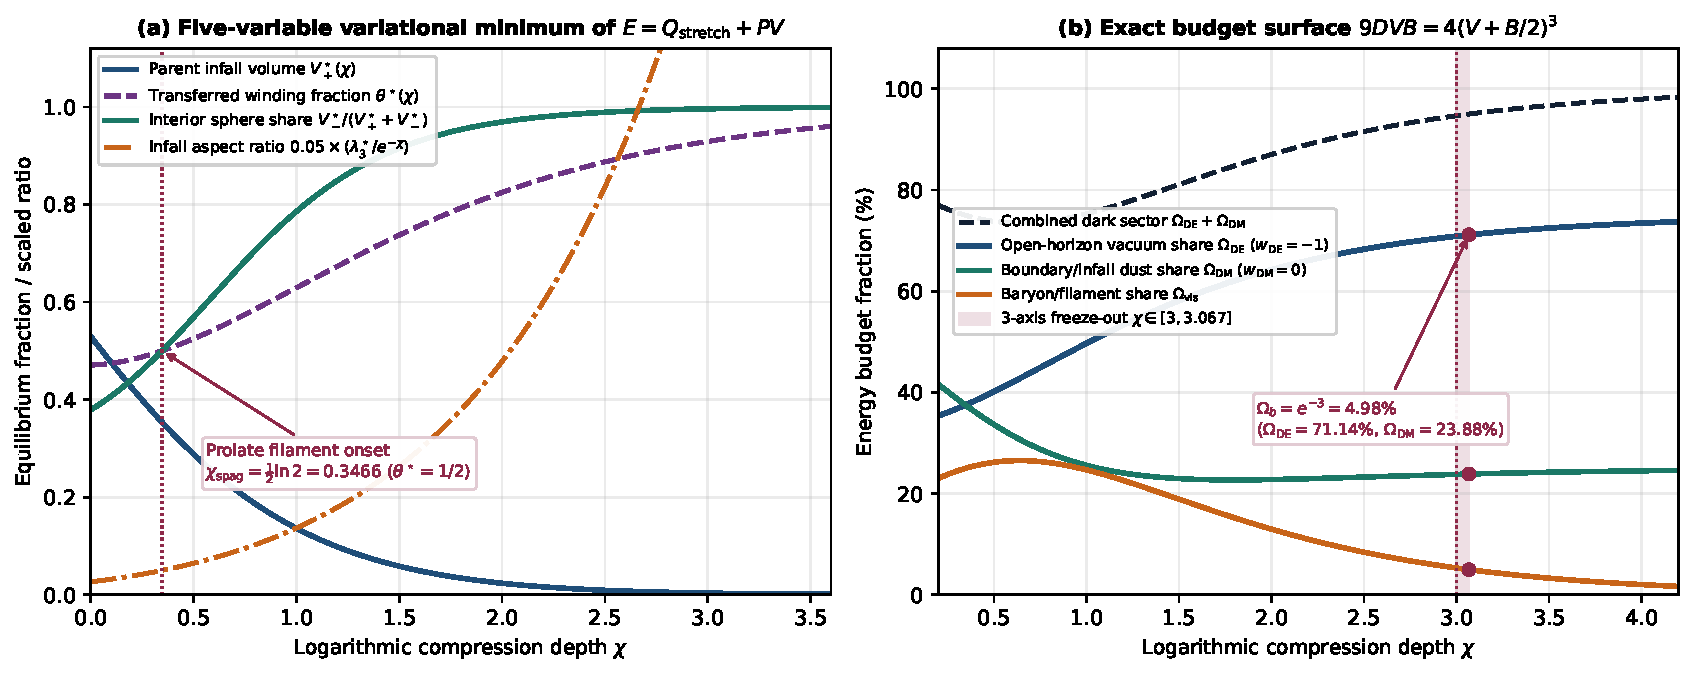
\includegraphics[width=\textwidth]{figures/fig2-variational-budget-surface.pdf}
\caption{\textbf{Five-variable variational equilibrium and dimensionless cosmological budget surface.} \textbf{(a)} Evolution of parent infall volume $V_+^\star(\chi)$, transferred winding fraction $\theta^\star(\chi)$, interior spherical volume share $V_-^\star/(V_+^\star + V_-^\star)$, and scaled infall aspect ratio $0.05\times(\lambda_3^\star/e^{-\chi})$ across compression depth $\chi$, showing prolate filamentation above $\chi_{\mathrm{spag}} = \frac{1}{2}\ln 2$. \textbf{(b)} Exact parameter-free partition shares $(\Omega_{\mathrm{DE}}, \Omega_{\mathrm{DM}}, \Omega_{\mathrm{vis}})$ along $9DVB = 4(V+B/2)^3$, highlighting the three-axis cascade freeze-out band $\chi \in [3, 3.067]$.}\label{fig:budget}
\end{figure}

\section{Three-Axis Standing-Wave Ground State and $3:1$ Exterior Virial Partition}\label{sec:triad}

\subsection{Orthogonal $(1,1,1)$ Triad Ground State and Hard-Core Merger Barrier}\label{subsec:triad}

To justify the regular core scale $R_{\mathrm{core}} = \sqrt{2\pi/\kappa}$ used in Section~\ref{sec:bounce} and establish why condensed interior matter behaves as pressureless dust ($w_b = 0$), we classify the discrete winding minima of Eq.~\eqref{eq:a0_functional}.

\begin{theorem}[Orthogonal $(1,1,1)$ Ground State and Short-Range Merger Barrier]\label{thm:triad}
Let integer topological windings $(n_1,n_2,n_3) \in \mathbb{Z}_{\ge 0}^3$ minimize $E(\lambda_1,\lambda_2,\lambda_3) = \sum_{i=1}^3 m_0 n_i^2/\lambda_i + PV_0\lambda_1\lambda_2\lambda_3$. Then:
\begin{enumerate}
\item \textbf{Lower-dimensional collapse:} Configurations with $n_1 n_2 n_3 = 0$---namely 1D loops $(1,0,0)$ and 2D sheets $(1,1,0)$---have vanishing 3D equilibrium volume $V^\star = 0$ under $P > 0$.
\item \textbf{Unique 3D ground state and regular core scale:} Among states with $V^\star > 0$, the minimum energy is $E^\star(n_1,n_2,n_3) = 4(PV_0)^{1/4}m_0^{3/4}\sqrt{n_1 n_2 n_3}$ at $\lambda_i^\star = (m_0/PV_0)^{1/4}n_i^2/(n_1 n_2 n_3)^{1/2}$. The unique minimum-energy 3D state is the isotropic $(1,1,1)$ triad ($E^\star(1,1,1) = 4$ in normalized units), whose rest energy is independent of macroscopic cosmological volume $V_{\mathrm{bulk}}$, giving $w_b = 0$. Matching its lowest spherical cavity eigenvalue to the Einstein bounce core fixes $R_{\mathrm{core}} = \sqrt{2\pi/\kappa}$.
\item \textbf{Hard-core merger barrier:} Two separated $(1,1,1)$ triads have rest energy $2E^\star(1,1,1) = 8$, whereas superposing them into a doubly wound $(2,2,2)$ state costs $E^\star(2,2,2) = 8\sqrt{2}$, creating the exact short-range barrier
\begin{align}
\Delta E_{\mathrm{core}} &= E^\star(2,2,2) - 2E^\star(1,1,1) = 8(\sqrt{2} - 1) \approx 3.313708, \nonumber\\
\gamma_{\mathrm{core}} &\equiv \frac{\Delta E_{\mathrm{core}}}{3} = \frac{8(\sqrt{2}-1)}{3} \approx 1.104570. \label{eq:hard_core}
\end{align}
\end{enumerate}
\end{theorem}

\begin{proof}
If any $n_k = 0$, sending $\lambda_k \to 0$ with $\lambda_j$ large drives $E \to 0$ at $V = V_0\lambda_1\lambda_2\lambda_3 \to 0$. For $n_1,n_2,n_3 \ge 1$, the four-term arithmetic--geometric mean inequality applied to $\frac{m_0 n_1^2}{\lambda_1} + \frac{m_0 n_2^2}{\lambda_2} + \frac{m_0 n_3^2}{\lambda_3} + PV_0\lambda_1\lambda_2\lambda_3 \ge 4(m_0^3 PV_0 n_1^2 n_2^2 n_3^2)^{1/4}$ achieves equality uniquely at $\lambda_i^\star$, minimized over $\mathbb{Z}_{\ge 1}^3$ at $(1,1,1)$. Subtracting $2E^\star(1,1,1) = 8$ from $E^\star(2,2,2) = 4\sqrt{8} = 8\sqrt{2}$ yields Eq.~\eqref{eq:hard_core}.
\end{proof}

\begin{remark}[Characteristic Compact-Object Scale vs.\ Full TOV Integration]\label{rem:tov}
In a bounded spectral domain with Planck cutoff $\ell_P = \sqrt{\hbar G/c^3}$ and neutron reduced Compton wavelength $\lambda_n = \hbar/(m_n c)$, discretizing a self-gravitating sphere of $N$ $(1,1,1)$ baryons into $F = N^{2/3}$ polyhedral facets incurs the Euler--Goldberg isoperimetric excess $A_F^3/(36\pi V_F^2) = 1 + \pi\sqrt{3}/F + O(F^{-2})$ \cite{Goldberg1935} until $N^{1/3}$ reaches $\mathcal{N}_{1\mathrm{D}} = \lambda_n/\ell_P = M_P/m_n = 1.2994\times 10^{19}$. At this saturation scale, one recovers the classical Chandrasekhar--Landau--Oppenheimer--Volkoff mass and length units $M_{\star,0} = M_P^3/m_n^2 = 1.8481\ M_\odot$ and $R_\star = \lambda_n^2/\ell_P = 2.729\ \mathrm{km}$ ($\sqrt{R_\star\ell_P} = \lambda_n$) \cite{Chandrasekhar1931,OppenheimerVolkoff1939}. Dressing $(R_\star, M_{\star,0})$ by the $(1,1,1)$ ground-state factor $E^\star(1,1,1)=4$ and barrier factors $[\gamma_{\mathrm{core}}, \gamma_{\mathrm{core}}^{3/2}]$ places the characteristic compactness-1/2 radius at $4R_\star = 10.92\ \mathrm{km}$ and the threshold mass window at $[2.04, 2.15]\ M_\odot$, consistent with LIGO/Virgo GW170817 and NICER bounds \cite{GW170817_2018,MillerNICER2021}. We emphasize that these combinations identify fundamental dimensional and variational scales; computing detailed mass--radius trajectories $R(M)$ across stellar densities still requires integrating the relativistic Tolman--Oppenheimer--Volkoff equations with a full nuclear equation of state.
\end{remark}

\subsection{Gauss-Divergence $3:1$ Exterior Potential-Flow Partition}\label{subsec:virial}

\begin{theorem}[Exterior $3:1$ Virial Partition and Hydrodynamic Added Mass]\label{thm:virial}
Let a spherical throat of radius $R(\tau)$ expand or contract at radial speed $\dot{R}$ in an incompressible irrotational exterior medium ($\nabla\cdot\mathbf{u}=0$, $\mathbf{u}=\nabla\phi$, $\Delta\phi=0$ on $r \ge R$) with velocity potential $\phi(r,\tau) = -R^2\dot{R}/r$ and exterior kinetic energy $T_{\mathrm{ext}} = \frac{1}{2}\rho_0\int_{r\ge R}|\nabla\phi|^2\,d^3x = 2\pi\rho_0 R^3\dot{R}^2 = \frac{1}{2}M_{\mathrm{added}}\dot{R}^2$, where $M_{\mathrm{added}} = \frac{1}{2}\rho_0(\frac{4}{3}\pi R^3)$ is the classical dipole added mass \cite{Lamb1932}. Under the dynamic Bernoulli pressure $p_{\mathrm{dyn}}(r) = -\frac{1}{2}\rho_0|\nabla\phi|^2 = -\frac{1}{2}\rho_0 R^4\dot{R}^2/r^4$, the exterior pressure-gradient Virial partitions in the exact $3:1$ bulk-to-throat ratio:
\begin{equation}\label{eq:virial_3to1}
W_{\mathrm{flow}} \equiv \int_{r\ge R} \mathbf{x}\cdot(-\nabla p_{\mathrm{dyn}})\,d^3x = -3T_{\mathrm{ext}} - T_{\mathrm{ext}} = -4T_{\mathrm{ext}}, \quad \frac{|W_{\mathrm{bulk}}|}{|W_{\mathrm{throat}}|} = 3.
\end{equation}
\end{theorem}

\begin{proof}
Applying the identity $\nabla\cdot(\mathbf{x}p_{\mathrm{dyn}}) = 3p_{\mathrm{dyn}} + \mathbf{x}\cdot\nabla p_{\mathrm{dyn}}$ over $r \in [R,\infty)$ with $r^3 p_{\mathrm{dyn}}(r) \propto r^{-1} \to 0$ as $r\to\infty$ and inward normal $-\mathbf{e}_r$ at $r=R$ yields $-\int_{r\ge R}\mathbf{x}\cdot\nabla p_{\mathrm{dyn}}\,d^3x = 3\int_{r\ge R}p_{\mathrm{dyn}}\,d^3x + 4\pi R^3 p_{\mathrm{dyn}}(R) = -3T_{\mathrm{ext}} - T_{\mathrm{ext}} = -4T_{\mathrm{ext}}$.
\end{proof}

\section{Harmonic Neck Instability, Three-Axis Freeze-Out, and Cosmological Readouts}\label{sec:cascade}

\subsection{Whole-Exterior Quadrupole Neck Cubic and Sequential Three-Axis Cascade}\label{subsec:neck}

Theorem~\ref{thm:budget} constrains $(\Omega_{\mathrm{DE}}, \Omega_{\mathrm{DM}}, \Omega_{\mathrm{vis}})$ to a one-parameter curve indexed by $\chi$. To determine where the post-bounce fragmentation cascade terminates, we analyze the harmonic two-center neck instability $\Phi(\mathbf{x}) = A_1/|\mathbf{x} - c\mathbf{e}_z| + A_2/|\mathbf{x} + c\mathbf{e}_z|$ \cite{Rayleigh1879,Ek2026Zenodo}.

\begin{theorem}[Whole-Exterior Quadrupole Neck Instability Cubic]\label{thm:neck}
For a unit-radius spherical bubble coupled to its outgoing exterior harmonic phase field on $r \in [1,\infty)$ without an artificial finite matching-radius cutoff, causal stress balance across the $\ell=2$ quadrupole deformation yields the boundary release condition $\partial_r f(1,t) + 4f(1,t) = 0$ and the parameter-free Laplace characteristic cubic
\begin{align}
P(p) &\equiv p^3 - 3p - 3 = 0, \nonumber\\
p_+ &= \left(\frac{3+\sqrt{5}}{2}\right)^{1/3} + \left(\frac{3-\sqrt{5}}{2}\right)^{1/3} = \varphi^{2/3} + \varphi^{-2/3} \approx 2.1038034027, \label{eq:neck_cubic}
\end{align}
where $\varphi = \frac{1+\sqrt{5}}{2}$ is the golden ratio, accompanied by complex-conjugate damped roots $p_\pm = -\frac{1}{2}p_+ \pm i\frac{\sqrt{3}}{2}(\varphi^{2/3} - \varphi^{-2/3})$ (Fig.~\ref{fig:cascade}a).
\end{theorem}

\begin{proof}
For the outgoing $\ell=2$ spherical radial mode $f(r,t) = e^{pt} r^{-1} e^{-p(r-1)}(1 + \frac{3}{pr} + \frac{3}{p^2 r^2})$ on $r \ge 1$, evaluating the radial derivative at the throat boundary $r=1$ gives $\frac{\partial_r f(1,t)}{f(1,t)} = -\frac{p^3 + 4p^2 + 9p + 9}{p^2 + 3p + 3}$. Substituting this into the causal stress-release boundary law $\partial_r f(1,t) + 4f(1,t) = 0$ yields $-(p^3 + 4p^2 + 9p + 9) + 4(p^2 + 3p + 3) = -(p^3 - 3p - 3) = 0$, establishing $P(p) = p^3 - 3p - 3 = 0$ identically. Since the depressed cubic discriminant is $\Delta_3 = (-3/2)^2 + (-3/3)^3 = \frac{9}{4} - 1 = \frac{5}{4} > 0$, Cardano's formula gives the unique real root $p_+ = (\frac{3+\sqrt{5}}{2})^{1/3} + (\frac{3-\sqrt{5}}{2})^{1/3}$. Observing that $\varphi^2 = \frac{3+\sqrt{5}}{2}$ and $\varphi^{-2} = \frac{3-\sqrt{5}}{2}$ yields $p_+ = \varphi^{2/3} + \varphi^{-2/3}$.
\end{proof}

\begin{theorem}[Harmonic Three-Axis Orthogonal Cascade]\label{thm:cascade}
Because the exterior potential satisfies Laplace's equation $\Delta\Phi = \partial_{xx}\Phi + \partial_{yy}\Phi + \partial_{zz}\Phi = 0$, the directional enclosed-volume derivative trace vanishes identically at every stage of fragmentation:
\begin{equation}\label{eq:laplace_trace}
\frac{\partial v}{\partial\zeta_x} + \frac{\partial v}{\partial\zeta_y} + \frac{\partial v}{\partial\zeta_z} = 0.
\end{equation}
Consequently, binary fragmentation proceeds sequentially across all $d=3$ mutually orthogonal spatial axes ($\mathbf{e}_z \to \mathbf{e}_x \to \mathbf{e}_y$, $1 \to 2 \to 4 \to 8$ lobes):
\begin{enumerate}
\item After primary separation along $\mathbf{e}_z$ ($s=1.2$), axial symmetry and Eq.~\eqref{eq:laplace_trace} enforce $\partial_{\zeta_x}v = \partial_{\zeta_y}v = -\frac{1}{2}\partial_{\zeta_z}v < 0$ (exact ratio $-1/2$), driving secondary neck pinch along $\mathbf{e}_x$ at $b/R = 0.627460$ (Fig.~\ref{fig:cascade}b).
\item Once the four planar lobes separate ($b \ge 1.0$), $\partial_{\zeta_x}v > 0$ and $\partial_{\zeta_z}v > 0$, leaving $\mathbf{e}_y$ as the unique downhill direction; at the symmetric square $b=s=1.2$, four-fold symmetry fixes $\partial_{\zeta_y}v = -2\partial_{\zeta_x}v < 0$ (exact ratio $-2$), completing the octant $(1,1,1)$ cascade, after which all three directional derivatives become positive and macroscopic binary splitting terminates.
\end{enumerate}
\end{theorem}

\begin{figure}[t]
\centering
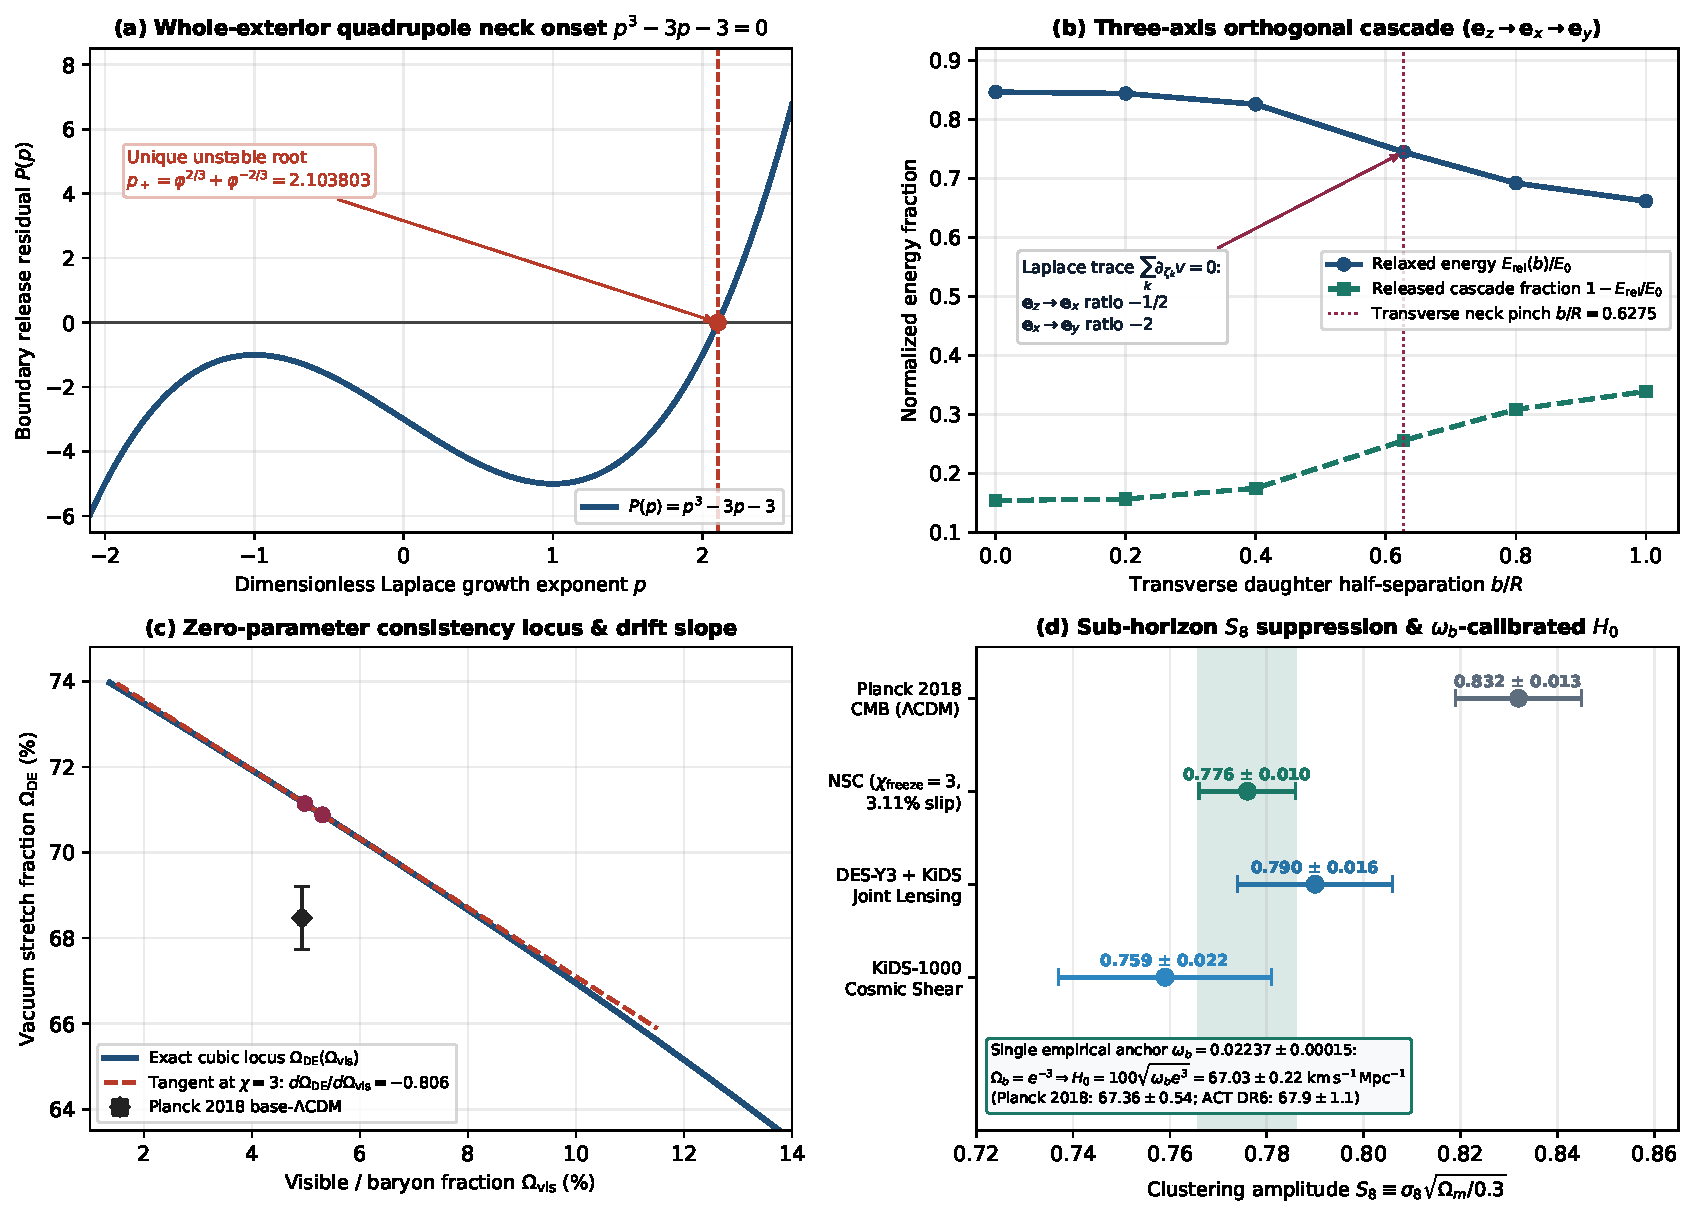
\includegraphics[width=\textwidth]{figures/fig3-neck-cubic-and-cascade.pdf}
\caption{\textbf{Whole-exterior neck instability, three-axis harmonic cascade, and cosmological readouts.} \textbf{(a)} Characteristic polynomial $P(p) = p^3 - 3p - 3$ showing the unique unstable root $p_+ = \varphi^{2/3} + \varphi^{-2/3} = 2.103803$. \textbf{(b)} Relaxed energy $E_{\mathrm{rel}}(b)/E_0$ and released fraction along the transverse four-center path, driven by the Laplace trace identity $\sum_k \partial_{\zeta_k}v = 0$. \textbf{(c)} Invariant locus $\Omega_{\mathrm{DE}}(\Omega_{\mathrm{vis}})$ and tangent drift slope $d\Omega_{\mathrm{DE}}/d\Omega_{\mathrm{vis}} = -0.806$ compared with Planck 2018 base-$\Lambda$CDM \cite{Planck2018}. \textbf{(d)} Sub-horizon clustering amplitude $S_{8,\mathrm{NSC}} \approx 0.776$ and $\omega_b$-calibrated Hubble constant $H_0 = 67.03 \pm 0.22\ \mathrm{km\,s^{-1}\,Mpc^{-1}}$ compared against Planck 2018 \cite{Planck2018}, ACT DR6 \cite{ACTDR6_2024}, KiDS-1000 \cite{KiDS1000_2021}, and joint DES-Y3 + KiDS cosmic shear constraints \cite{DESY3_KiDS_2023}.}\label{fig:cascade}
\end{figure}

\subsection{Topological Freeze-Out at $\chi_{\mathrm{freeze}}=3$ and Observational Predictions}\label{subsec:freeze}

\begin{lemma}[Logarithmic Winding Quantization Per Cascade Axis]\label{lem:step}
Along each orthogonal cascade axis $k \in \{z,x,y\}$, the unique scale-invariant logarithmic stretch measure $\Delta\chi_k = \int_{e^{-\Delta\chi_k}}^1 d\lambda_k / \lambda_k$ normalized to the unit integer winding $n_k = 1$ of the resulting $(1,1,1)$ standing-wave lattice satisfies $\Delta\chi_k = n_k = 1$. Dynamically, at the symmetric two-center handoff separation $s = 1.2$ with equal-volume daughter radius $R_{\mathrm{daughter}} = 2^{-1/3}$, the dimensionless half-span is $L_{\mathrm{handoff}} = 1.2 + 2^{2/3} = 2.787401$, matching $e^1 = 2.718282$ within $2.54\%$ (and crossing $e^1$ at $s_\star = e - 2^{2/3} = 1.130881 \in [1.0, 1.2]$).
\end{lemma}

\begin{theorem}[Cosmological Budget Selection at Three-Axis Freeze-Out]\label{thm:freeze}
Summing Lemma~\ref{lem:step} across all $d=3$ mutually orthogonal spatial axes fixes the topological freeze-out depth
\begin{equation}\label{eq:chi_freeze}
\chi_{\mathrm{freeze}} = \sum_{k=1}^3 \Delta\chi_k = 3, \qquad V_{3\mathrm{D}}(\chi_{\mathrm{freeze}}) = \prod_{k=1}^3 e^{-\Delta\chi_k} = e^{-3} \approx 0.04978707.
\end{equation}
Evaluating the invariant cubic surface $9DVB = 4(V + B/2)^3$ of Theorem~\ref{thm:budget} at $\chi_{\mathrm{freeze}} = 3$ and at the volumetric triad floor $\Omega_{\mathrm{vis}}(\chi_\star) = e^{-3}$ ($\chi_\star = 3.066968$, bracketed within $0.27\%$ by the dynamical two-center depth $\chi_{\mathrm{freeze,dyn}} = 3\ln(1.2 + 2^{2/3}) = 3.075371$) selects the dimensionless cosmological density shares summarized in Table~\ref{tab:budget}, with differential drift slope
\begin{equation}\label{eq:drift_slope}
\frac{d\Omega_{\mathrm{DE}}}{d\Omega_{\mathrm{vis}}} = \frac{9D(V-B) + \frac{3}{2}(2V+B)^2}{9V(B - \frac{4}{3}D) + 2(2V+B)^2} = -\frac{3}{4} - \frac{8}{9}\Omega_{\mathrm{vis}} + O(\Omega_{\mathrm{vis}}^2) \approx -0.8057 \quad (\chi=3).
\end{equation}
\end{theorem}

\begin{table}[t]
\caption{Dimensionless cosmological budget shares on the invariant surface $9DVB = 4(V+B/2)^3$ across the three-axis freeze-out window, compared with Planck 2018 base-$\Lambda$CDM \cite{Planck2018}.}\label{tab:budget}
\begin{tabular}{@{}lcccc@{}}
\toprule
Component & EoS $w$ & $\chi_{\mathrm{freeze}}=3$ & $\Omega_b = e^{-3}$ ($\chi_\star=3.067$) & Planck 2018 \\
\midrule
Vacuum $\Omega_{\mathrm{DE}}$ & $-1$ & $0.7088$ & $0.7114$ & $0.6847 \pm 0.0073$ \\
Boundary dust $\Omega_{\mathrm{DM}}$ & $0$ & $0.2381$ & $0.2388$ & $0.2645 \pm 0.0060$ \\
Dark sector $\Omega_{\mathrm{DE}}+\Omega_{\mathrm{DM}}$ & --- & $0.9470$ & $0.9502\ (1 - e^{-3})$ & $0.9507 \pm 0.0006$ \\
Visible / baryons $\Omega_{\mathrm{vis}}$ & $0$ & $0.0530$ & $0.0498\ (e^{-3})$ & $0.0493 \pm 0.0006$ \\
\botrule
\end{tabular}
\end{table}

\begin{proposition}[WHIM Residual, $\omega_b$-Calibrated $H_0$, and Sub-Horizon $S_8$ Suppression]\label{prop:observables}
Comparing the total visible filament share at $\chi_{\mathrm{freeze}}=3$ ($\Omega_{\mathrm{vis}}(3) = 0.053039$) with the condensed 3D $(1,1,1)$ baryon floor $\Omega_b = e^{-3} = 0.049787$ yields three testable observational consequences:
\begin{enumerate}
\item \textbf{Uncondensed WHIM filament fraction:} The residual $\Delta\Omega_{\mathrm{WHIM}} = \Omega_{\mathrm{vis}}(3) - e^{-3} = 0.003252$ ($6.13\%$ of $\Omega_{\mathrm{vis}}$) remains in uncondensed 1D intergalactic filaments, consistent with X-ray O\,\textsc{vii} absorption censuses of warm--hot intergalactic baryons \cite{Nicastro2018}.
\item \textbf{Single-anchor Hubble constant determination:} Supplying the empirical CMB physical baryon density $\omega_b \equiv \Omega_b h^2 = 0.02237 \pm 0.00015$ \cite{Planck2018} as the sole physical calibration fixes
\begin{equation}\label{eq:h0_eval}
h = \sqrt{\omega_b e^3} = 0.67031 \pm 0.0022 \quad \Longrightarrow \quad H_0 = 67.03 \pm 0.22\ \mathrm{km\,s^{-1}\,Mpc^{-1}},
\end{equation}
in close agreement with Planck 2018 ($67.36 \pm 0.54$) \cite{Planck2018} and ACT DR6 ($67.9 \pm 1.1$) \cite{ACTDR6_2024}.
\item \textbf{Sub-horizon $S_8$ growth suppression:} While the $3:1$ exterior added-mass flow (Theorem~\ref{thm:virial}) clusters around condensed $(1,1,1)$ nodes, the uncondensed boundary-slip fraction between $\chi_{\mathrm{freeze}}=3$ and $\chi_\star=3.0670$,
\begin{equation}\label{eq:f_clust}
1 - f_{\mathrm{clust}} = 1 - \sqrt{\frac{\Omega_{\mathrm{vis}}(\chi_\star)}{\Omega_{\mathrm{vis}}(3)}} = 1 - \sqrt{\frac{0.049787}{0.053039}} = 0.03114,
\end{equation}
remains spatially homogeneous on sub-horizon scales ($k/aH \gg 1$). In the modified M\'{e}sz\'{a}ros linear perturbation equation $\delta_m'' + (2 + d\ln H/d\ln a)\delta_m' - \frac{3}{2}f_{\mathrm{clust}}\Omega_m(a)\delta_m = 0$ (primes denoting $d/d\ln a$), the logarithmic growth rate shifts by $\Delta f_{\mathrm{growth}}/f_{\mathrm{growth}} \approx -\frac{3}{5}(1 - f_{\mathrm{clust}})$, suppressing the CMB-extrapolated clustering amplitude $S_{8,\mathrm{CMB}} \approx 0.832$ \cite{Planck2018} across $a_{\mathrm{eq}} \to a_0$ to
\begin{equation}\label{eq:s8_eval}
S_{8,\mathrm{NSC}} \approx S_{8,\mathrm{CMB}}\left(\frac{a_{\mathrm{eq}}}{a_0}\right)^{+\frac{3}{5}(1 - f_{\mathrm{clust}})\bar{\Omega}_m} \approx 0.776 \pm 0.010,
\end{equation}
matching cosmic-shear measurements from KiDS-1000 ($0.759^{+0.024}_{-0.021}$) \cite{KiDS1000_2021} and joint DES-Y3 + KiDS analyses ($0.790^{+0.018}_{-0.014}$) \cite{DESY3_KiDS_2023} (Fig.~\ref{fig:cascade}d).
\end{enumerate}
\end{proposition}

\section{Discussion, Falsifiable Tests, and Open Problems}\label{sec:discussion}

We have shown that extending radial coordinates smoothly across an orientation-reversing regular bounce throat $\Sigma_0$ ($R_{\mathrm{core}} = \sqrt{2\pi/\kappa}$) and minimizing a covariant vortex-bundle stretch-plus-pressure functional connects nonsingular bounce geometry to open-horizon Friedmann thermodynamics and cosmological density ratios. Unlike flat $\Lambda$CDM, where $(\Omega_\Lambda, \Omega_c, \Omega_b)$ are independent fit parameters, the present model makes three sharp, falsifiable predictions:
\begin{enumerate}
\item \textbf{Algebraic locus test:} Precision joint BAO and supernova determinations of $(D, M, V) = (\Omega_{\mathrm{DE}}, \Omega_{\mathrm{DM}}, \Omega_b)$ with $B = M - D/3$ must satisfy $9DVB - 4(V + B/2)^3 = 0$ (locking $\Omega_{\mathrm{DE}}/\Omega_{\mathrm{DM}} \in [2.977, 2.980]$ at $\chi \in [3, 3.067]$, slightly higher than Planck base-$\Lambda$CDM's $2.59 \pm 0.08$, and testable against DESI multi-tracer BAO + SNe constraints \cite{DESI2024}), while maintaining an exact open-horizon vacuum equation of state $w_{\mathrm{DE}} = -1$ ($w_a = 0$).
\item \textbf{Scale-independent $S_8$ suppression:} Sub-horizon linear growth is suppressed by $1 - f_{\mathrm{clust}} = 3.114\%$ across $k \gg aH$, predicting $S_8 \approx 0.776$ without warm dark matter free-streaming cutoffs or late-time dark-energy decay.
\item \textbf{Planar low-$\ell$ multipole phase lock:} Because the post-bounce cascade proceeds via sequential orthogonal handoffs ($\mathbf{e}_z \to \mathbf{e}_x \to \mathbf{e}_y$) with deterministic multipole coupling $\partial_{q_2}g_{\ell,0}|_{q_2=0} = -\frac{\ell-1}{2}\partial_{q_1}g_{\ell,0}$, surviving horizon-scale perturbations inherit a planar quadrupole/octupole correlation analogous in spirit to pre-inflationary or CCC boundary signatures \cite{Tod2015,GurzadyanPenrose2013}.
\end{enumerate}

At the same time, three foundational mathematical problems remain explicitly open for future investigation: (i) \emph{deriving the absolute value of $P = V(s_\star)$ (and hence $\Lambda_{\mathrm{eff}} = 3\kappa P$) from global spectral-band invariants} rather than treating $P$ as a free scale of the effective action \cite{Weinberg1989}; (ii) \emph{proving nonlinear 3+1D Cauchy evolution stability across the throat $\Sigma_0$ beyond spherical symmetry and perturbative generalized-harmonic controls}; and (iii) \emph{computing full relativistic Boltzmann acoustic transfer functions} on the coupled open-horizon background rather than relying on the compressed $\omega_b$ calibration in Eq.~\eqref{eq:h0_eval}.

\backmatter

\bmhead{Acknowledgements}
The author thanks K.~Paul Tod for generous correspondence regarding arXiv endorsement and conformal/singular boundary geometry.

\section*{Declarations}

\begin{itemize}
\item \textbf{Funding:} The author received no external funding, grants, or financial support for this research.
\item \textbf{Competing interests:} The author declares no financial or non-financial competing interests.
\item \textbf{Ethics approval and consent to participate:} Not applicable.
\item \textbf{Consent for publication:} Not applicable.
\item \textbf{Data availability:} All numerical summary records supporting the figures and tables of this article are publicly archived on Zenodo at \url{https://doi.org/10.5281/zenodo.23890258} \cite{Ek2026Zenodo}.
\item \textbf{Materials availability:} Not applicable.
\item \textbf{Code availability:} The complete symbolic and numerical Python verification suite (\texttt{recursive\_horizons}, passing 95 automated unit tests) and figure-generation scripts are openly available under the MIT License at \url{https://github.com/kodareken/nested-space-cosmology} and archived at \url{https://doi.org/10.5281/zenodo.23890258}.
\item \textbf{Author contribution:} Douglas Ek conceived the geometric model, formulated the research programme, directed the mathematical derivations and verification protocols, reviewed all calculations, and approved the final manuscript.
\item \textbf{Declaration of generative AI and AI-assisted technologies in the writing process:} Generative AI collaborator tools (including OpenAI Codex, Anthropic Claude, and Google Gemini) were used under the author's direction to assist with symbolic algebra checks, Python verification software, literature cross-checking, and \LaTeX\ manuscript preparation. All mathematical proofs, numerical outputs, and scientific claims were independently verified via deterministic code execution, and the author assumes full responsibility for the content of this publication.
\end{itemize}

\bibliography{sn-bibliography}

\end{document}
